%!TEX program = xelatex
% 完整编译: xelatex -> biber/bibtex -> xelatex -> xelatex
\documentclass[lang=cn,11pt,a4paper]{paper}

\title{编译原理与技术 实验一:词法分析程序的设计与实现 \\ 实验报告}
\author{张梓良 \\ 2021212484}
\institute{北京邮电大学 \\ 计算机科学与技术}

\date{\zhtoday}


% 本文档命令
\usepackage{array}
\newcommand{\ccr}[1]{\makecell{{\color{#1}\rule{1cm}{1cm}}}}
\usepackage{xcolor}
% 定义可能使用到的颜色
\definecolor{CPPLight}  {HTML} {686868}
\definecolor{CPPSteel}  {HTML} {888888}
\definecolor{CPPDark}   {HTML} {262626}
\definecolor{CPPBlue}   {HTML} {4172A3}
\definecolor{CPPGreen}  {HTML} {487818}
\definecolor{CPPBrown}  {HTML} {A07040}
\definecolor{CPPRed}    {HTML} {AD4D3A}
\definecolor{CPPViolet} {HTML} {7040A0}
\definecolor{CPPGray}  {HTML} {B8B8B8}
\lstset{
    columns=fixed,       
    numbers=left,                                        % 在左侧显示行号
    frame=none,                                          % 不显示背景边框
    backgroundcolor=\color[RGB]{245,245,244},            % 设定背景颜色
    keywordstyle=\color[RGB]{40,40,255},                 % 设定关键字颜色
    numberstyle=\footnotesize\color{darkgray},           % 设定行号格式
    commentstyle=\it\color[RGB]{0,96,96},                % 设置代码注释的格式
    stringstyle=\rmfamily\slshape\color[RGB]{128,0,0},   % 设置字符串格式
    showstringspaces=false,                              % 不显示字符串中的空格
    language=c++,                                        % 设置语言
    morekeywords={alignas,continute,friend,register,true,alignof,decltype,goto,
    reinterpret_cast,try,asm,defult,if,return,typedef,auto,delete,inline,short,
    typeid,bool,do,int,signed,typename,break,double,long,sizeof,union,case,
    dynamic_cast,mutable,static,unsigned,catch,else,namespace,static_assert,using,
    char,enum,new,static_cast,virtual,char16_t,char32_t,explict,noexcept,struct,
    void,export,nullptr,switch,volatile,class,extern,operator,template,wchar_t,
    const,false,private,this,while,constexpr,float,protected,thread_local,
    const_cast,for,public,throw,std},
    emph={map,set,multimap,multiset,unordered_map,unordered_set,
    unordered_multiset,unordered_multimap,vector,string,list,deque,
    array,stack,forwared_list,iostream,memory,shared_ptr,unique_ptr,
    random,bitset,ostream,istream,cout,cin,endl,move,default_random_engine,
    uniform_int_distribution,iterator,algorithm,functional,bing,numeric,},
    emphstyle=\color{CPPViolet}, 
}

\begin{document}

\maketitle

\section{概述}

\subsection{实验内容及要求}

\begin{enumerate}
  \item 选定源语言,比如:\ \lstinline{C、Pascal、Python、Java}\ 等,任何一种语言均可。
  \item 可以识别出用源语言编写的源程序中的每个单词符号,并以记号的形式输出每个单词符号。
  \item 可以识别并跳过源程序中的注释。
  \item 可以统计源程序中的语句行数、各类单词的个数、以及字符总数,并输出统计结果。
  \item 检查源程序中存在的词法错误,并报告错误所在的位置。
  \item 对源程序中出现的错误进行适当的恢复,使词法分析可以继续进行,对源程序进行一次扫描,即可检查并报告源程序中存在的所有词法错误。
\end{enumerate}

\subsection{实验环境}

\begin{itemize}
    \item flex version 2.5.4
    \item cmake version 3.27.0-rc4
    \item gcc version 8.1.0
    \item Visual Studio Code 1.82.2
    \item OS: Windows\_NT x64 10.0.22621
\end{itemize}

\subsection{实验目的}

编写\ \lstinline{LEX}\ 源程序,利用\ \lstinline{LEX}\ 编译程序自动生成词法分析程序。

\section{程序设计说明}

\subsection{模块划分}

词法分析程序分为四个模块:\lstinline{token, error, output, lex}\ ,其中\ \lstinline{token}\ 模块定义了所需的数据结构,\ \lstinline{error}\ 模块对词法分析过程中遇到的错误词法进行输出,\ \lstinline{output}\ 模块将词法分析得到的结果输出,\ \lstinline{lex}\ 模块对输入的文件流进行词法分析并将前三个模块组装构成整个词法分析程序。模块间的调用关系如\ \textbf{图\ \ref{fig:模块调用关系}}\ 。

\begin{figure}[!htb]
    \centering
    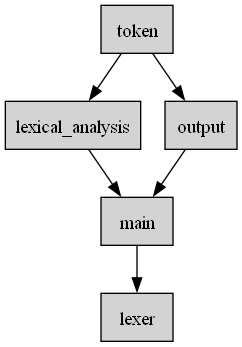
\includegraphics[
    width=0.3\textwidth]{module.png}
    \caption{模块调用关系}
    \label{fig:模块调用关系}
\end{figure}

\subsection{自定义数据结构}

\subsubsection{C语言记号类型}

\begin{lstlisting}
enum TokenType
{
    KEYWORD,              // 关键字
    ID,                   // 标志符
    STRING,               // 字符串常量
    CHAR,                 // 字符常量
    INT,                  // 整型常量
    UINT,                 // 无符号整型常量
    LONG,                 // 长整型常量
    ULONG,                // 无符号长整型
    LONGLONG,             // 长长整型常量
    ULONGLONG,            // 无符号长长整型常量
    FLOAT,                // 单精度浮点数
    DOUBLE,               // 双精度浮点数
    LONGDOUBLE,           // 长双精度浮点数
    RELATION_OPERATOR,    // 关系运算符
    ASSIGN_OPERATOR,      // 赋值运算符
    AGORITHM_OPERATOR,    // 算术运算符
    LOGICAL_OPERATOR,     // 逻辑运算符
    BITWISE_OPERATOR,     // 位运算符
    QUESTION_MARK,        //"?"
    COLON,                //":"
    SEMICOLON,            //";"
    LEFT_SQUARE_BRACKET,  //"["
    RIGHT_SQUARE_BRACKET, //"]"
    LEFT_PARENTHESE,      //"("
    RIGHT_PARENTHESE,     //")"
    LEFT_BRACE,           //"{"
    RIGHT_BRACE,          //"}"
    DOT,                  //"."
    COMMA,                //","
    ARROW,                //"->"
    ANNOTATION,           // 注释
};
\end{lstlisting}

采用\ \lstinline{enum}\ 类型存储记号类型,建立记号类型与非负整数之间的映射,便于词法分析时函数之间记号类型的传递。

\subsubsection{记号}

\begin{lstlisting}
struct Token
{
    enum TokenType type; // 记号类型
    char value[200];     // 记号值
    int line;            // 记号所在行数
    int column;          // 记号所在列数
};
\end{lstlisting}

一个记号中存储了记号类型、记号属性值、记号所在行数以及记号所在列数,其中记号类型采用先前已经自定义的数据类型。记号的表示形式为\ \lstinline{<line:column><type, value>}\ 。

\subsection{词法分析}

在\ \lstinline{lex.l}\ 中定义识别各类记号的正则表达式,再通过\ \lstinline{flex}\ 编译程序生成\ \lstinline{lex.yy.c}\ 文件来替代手工编写的\ \lstinline{lexical_analysis.cpp}\ 文件以实现词法分析程序。

\subsubsection{设计流程}

参考\ \lstinline{ISO_C99_definition}\ 中对各类记号的形式化定义画出识别各类记号的\ \lstinline{DFA},再根据\ \lstinline{DFA}\ 写出相应正则表达式。

\subsubsection{关键字的识别}

\ \lstinline{ISO_C99_definition}\ 中对关键字的定义如\ \textbf{图\ \ref{fig:C99对关键字的规定}}\ 所示。

\begin{figure}[!htb]
    \centering
    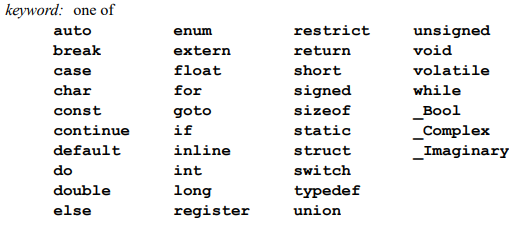
\includegraphics[
    width=0.7\textwidth]{keyword_def.png}
    \caption{C99对关键字的规定}
    \label{fig:C99对关键字的规定}
\end{figure}

据此写出正则表达式:

\begin{lstlisting}
keyword		(auto)|(break)|(case)|(char)|(const)|(continue)|(default)|(do)|(double)|(else)|(enum)|(extern)|(float)|(for)|(goto)|(if)|(inline)|(int)|(long)|(register)|(restrict)|(return)|(short)|(signed)|(sizeof)|(static)|(struct)|(switch)|(typedef)|(union)|(unsigned)|(void)|(volatile)|(while)|(_Bool)|(_Complex)|(_Complex)|(_Imaginary)    
\end{lstlisting}

\subsubsection{标识符的识别}

\ \lstinline{ISO_C99_definition}\ 中对标志符的定义如\ \textbf{图\ \ref{fig:C99对标识符的规定}}\ 所示。标识符只能由\ \lstinline{_ \ letter}\ 开头,可以包含\ \lstinline{_ \ letter \ digit}\ 。

\begin{figure}[!htb]
    \centering
    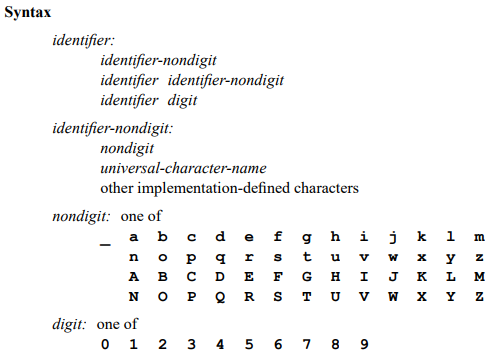
\includegraphics[
    width=0.7\textwidth]{identifier_def.png}
    \caption{C99对标识符的规定}
    \label{fig:C99对标识符的规定}
\end{figure}

采用\ \lstinline{dot}\ 语言实现识别标识符的\ \lstinline{DFA}\ :

\begin{lstlisting}
digraph G{
    rankdir=LR
    node[shape = circle]
    ID [shape = doublecircle]
    0 -> 1 [label = "- / letter"]
    1 -> 1 [label = "- / letter / digit"]
    1 -> ID [label = "other"]
}
\end{lstlisting}

据此写出正则表达式:

\begin{lstlisting}
letter    	[A-Za-z]
digit     	[0-9]
id        	({letter}|_)({letter}|{digit}|_)*
\end{lstlisting}

\subsubsection{常数的识别}
~\\
\textbf{常数可以按照两类标准分类:}
\begin{itemize}
    \item 以\ 0\ 开头还是非\ 0\ 数字开头还是\ .\ 开头
    \item 整型常数还是浮点型常数
\end{itemize}
~\\
\textbf{其中以\ 0\ 开头的常数又可以分为:}
\begin{itemize}
    \item 整数\ 0
    \item 以\ 0\ 开头的八进制整型常数
    \item 以\ 0\ 开头的十六进制整型常数
    \item 以\ 0\ 开头的浮点型常数
\end{itemize}
~\\
\textbf{其中以非\ 0\ 数字开头的常数又可以分为:}
\begin{itemize}
    \item 十进制整型常数
    \item 浮点型常数
\end{itemize}
~\\
\textbf{其中以\ .\ 开头的常数只能为浮点型常数}

~\\
\textbf{其中整形常数又可以分为:}
\begin{itemize}
    \item 十进制整型常数
    \item 八进制整型常数
    \item 十六进制整型常数
\end{itemize}
~\\
\textbf{其中浮点型常数又可以分为:}
\begin{itemize}
    \item\ \lstinline{float (f / F 后缀)}
    \item\ \lstinline{double (无后缀)}
    \item\ \lstinline{long double (l / L 后缀)}
\end{itemize}
~\\
\textbf{各种进制的整型常数又可以分为:}
\begin{itemize}
    \item\ \lstinline{int (无后缀)}
    \item\ \lstinline{unsigned int (u / U 后缀)}
    \item\ \lstinline{long (l / L 后缀)}
    \item\ \lstinline{unsigned long ((u / U) + (l / L) 后缀)}
    \item\ \lstinline{long long ((l / L) + (l / L) 后缀)}
    \item\ \lstinline{unsigned long long((u / U) + (l / L) + (l / L) 后缀)}
\end{itemize}
~\\

根据以上分类,采用\ \lstinline{dot}\ 语言对识别常数的\ \lstinline{DFA} 进行定义:

\begin{lstlisting}
digraph G{
    rankdir = LR
    splines = ortho
    node[shape = circle]
    DOT[shape = doublecircle, label = "DOT(4)"]
    INT[shape = doublecircle]
    UINT[shape = doublecircle, label = "UINT(30)"]
    ULONG[shape = doublecircle, label = "ULONG(32)"]
    ULONGLONG[shape = doublecircle]
    LONG[shape = doublecircle, label = "LONG(31)"]
    LONGLONG[shape = doublecircle]
    FLOAT[shape = doublecircle]
    DOUBLE[shape = doublecircle]
    LONGDOUBLE[shape = doublecircle]
    0 -> 2 [label = "digit(except 0)"]
    0 -> 3 [label = "0"]
    0 -> DOT [label = "."]
    2 -> 2 [label = "digit"]
    2 -> 22 [label = "."]
    2 -> 23 [label = "e / E"]
    2 -> UINT [label = "u / U"]
    2 -> LONG [label = "l / L"]
    UINT -> ULONG [label = "l / L"]
    ULONG -> ULONGLONG [label = "l / L"]
    LONG -> LONGLONG [label = "l / L"]
    2 -> INT [label = "INT"]
    22 -> 22 [label = "digit"]
    22 -> 23 [label = "e / E"]
    22 -> FLOAT [label = "f / F"]
    22 -> LONGDOUBLE [label = "l / L"]
    22 -> DOUBLE [label = "other"]
    23 -> 24 [label = "+ / -"]
    23 -> 25 [label = "digit"]
    24 -> 25 [label = "digit"]
    25 -> 25 [label = "digit"]
    25 -> FLOAT [label = "f / F"]
    25 -> LONGDOUBLE [label = "l / L"]
    25 -> DOUBLE [label = "other"]
    3 -> 22 [label = "."]
    3 -> 26 [label = "oct_digt"]
    3 -> 27 [label = "8 / 9"]
    3 -> 23 [label = "e / E"]
    3 -> 28 [label = "x / X"]
    3 -> INT [label = "other"]
    3 -> UINT [label = "u / U"]
    3 -> LONG [label = "l / L"]
    26 -> 27 [label = "8 / 9"]
    26 -> 26 [label = "oct_digit"]
    26 -> 23 [label = "e / E"]
    26 -> UINT [label = "u / U"]
    26 -> LONG [label = "l / L"]
    26 -> 22 [label = "."]
    27 -> 27 [label = "digit"]
    27 -> 22 [label = "."]
    27 -> 23 [label = "e / E"]
    28 -> 29 [label = "hex_digit"]
    29 -> 29 [label = "hex_digit"]
    29 -> INT [label = "other"]
    29 -> UINT [label = "u / U"]
    29 -> LONG [label = "l / L"]
    DOT -> 22 [label = "digit"]
}
\end{lstlisting}

据此写出正则表达式:

\begin{lstlisting}
digit     	[0-9]
octal_digit [0-7]
hex_digit 	[0-9a-fA-F]
int 		[1-9]{digit}*|0{octal_digit}*|0[xX]{hex_digit}+
uint		{int}(u|U)
long		{int}(l|L)
ulong		{int}(u|U)(l|L)
longlong	{int}(l|L)(l|L)
ulonglong	{int}(u|U)(l|L)(l|L)
double 		({digit}+\.{digit}*|\.{digit}+)([eE][\+\-]?{digit}+)?|{digit}+[eE][\+\-]?{digit}+
float		{double}(f|F)
longdouble	{double}(l|L)
\end{lstlisting}

\subsubsection{字符常量的识别}

\lstinline{DOT}\ 语言定义的识别字符常量的\ \lstinline{DFA}:

\begin{lstlisting}
digraph G{
    rankdir=LR
    splines = line
    node[shape = circle]
    CHAR [shape = doublecircle, fontsize = 10]
    ERROR [shape = doublecircle, label = "ERROR(21)", fontsize = 10]
    0 -> 7 [label = "'"]
    7 -> ERROR [label = "' / \\n / EOF "]
    7 -> 35 [label = "other"]
    7 -> 34 [label = "\\"]
    34 -> 35 [label = "legal escape characters"]
    35 -> CHAR [label = "'"]
}
\end{lstlisting}

据此写出正则表达式:

\begin{lstlisting}
char 		\'([^\'\n]|\\.)+\'
\end{lstlisting}

除此之外,我们需要考虑字符常量为空,eg.\lstinline{''},以及字符常量未闭合的错误情况,eg.\lstinline{'a}。

对以上错误情况进行匹配的正则表达式:

\begin{lstlisting}
unclosed_char			\'[^\'\n]*
empty_char				\'\'
\end{lstlisting}

\subsubsection{字符串常量的识别}

字符串常量的识别与字符常量的识别类似,同样需要考虑未闭合的错误情况,但字符串常量允许为空。

下面给出用\ \lstinline{DOT}\ 语言定义的识别字符串常量的\ \lstinline{DFA}:

\begin{lstlisting}
digraph G{
    rankdir=LR
    splines = line
    node[shape = circle]
    STRING [shape = doublecircle, fontsize = 10]
    ERROR [shape = doublecircle, label = "ERROR(21)", fontsize = 10]
    0 -> 6 [label = "\""]
    6 -> 6 [label = "other"]
    6 -> ERROR [label = "\\n / EOF"]
    6 -> 33 [label = "\\"]
    6 -> STRING [label = "\""]
    33 -> 6 [label = "legal escape characters"]
}
\end{lstlisting}

据此写出正则表达式:

\begin{lstlisting}
str			\"([^\"\n]|\\.)*\"
unclosed_string			\"[^\"\n]*
\end{lstlisting}

\subsubsection{运算符的识别}

运算符分为五大类:\lstinline{RELATION_OPERATOR, ASSIGN_OPERATOR, AGORITHM_OPERATOR, LOGICAL_OPERATOR, BITWISE_OPERATOR}

据此写出正则表达式:

\begin{lstlisting}
relation	(\<)|(\>)|(\<=)|(\>=)|(==)|(!=)
assign 		(=)|(\+=)|(\-=)|(\*=)|(\/=)|(\%=)|(&=)|(\|=)|(\^=)|(\<\<=)|(\>\>=)
agorithm 	(\+)|(\-)|(\*)|(\/)|(\%)|(\+\+)|(\-\-)
logical		(&&)|(\|\|)|(!)
bitwise		(&)|(\|)|(\^)|(~)|(\<\<)|(\>\>)
\end{lstlisting}

\subsubsection{注释的识别}

注释分为单行注释和多行注释,二者都以\ \lstinline{/}\ 开头。单行注释遇到\ \lstinline{\n}\ 或\ \lstinline{EOF}\ 结束;多行注释当匹配到对应的\ \lstinline{*/}\ 时结束,因此需要进行闭合检测,若读到文件末尾还没有与\ \lstinline{/*}\ 匹配的\ \lstinline{*/},就输出多行注释未闭合的错误。

下面给出用\ \lstinline{DOT}\ 语言定义的识别注释的\ \lstinline{DFA}:

\begin{lstlisting}
digraph G{
    rankdir=LR
    node[shape = circle]
    ANNOTATION [shape = doublecircle, fontsize = 10]
    0 -> 11 [label = "/"]
    11 -> 36 [label = "/"]
    11 -> 37 [label = "*"]
    36 -> 36 [label = "other"]
    36 -> ANNOTATION [label = "\\n / EOF"]
    37 -> 37 [label = "other"]
    37 -> 38 [label = "*"]
    38 -> 37 [label = "other"]
    38 -> 38 [label = "*"]
    38 -> ANNOTATION [label = "/"]
}
\end{lstlisting}

据此写出正则表达式:

\begin{lstlisting}
singleline_annotation		(\/\/)[^\n]*
multiline_annotation		(\/\*)(.|\n)*(\*\/)

unclosed_annotation		(\/\*)(.*)
\end{lstlisting}

\subsubsection{其他记号的识别}

其他记号的识别较为简单,直接在翻译规则部分写出即可。

\subsection{词法错误}

\subsubsection{“错误”类型的定义}

\begin{lstlisting}
enum ErrorType
{
    UNKNOWN_SYMBOL,     // 未知符号
    UNCLOSED_STRING,    // 未闭合字符串
    UNCLOSED_CHAR,      // 未闭合字符
    EMPTY_CHAR,         // 空字符
    UNCLOSED_ANNOTATION // 未闭合注释
};
\end{lstlisting}

\subsubsection{“错误”的正则匹配}

\begin{lstlisting}
unclosed_string			\"[^\"\n]*
unclosed_char			\'[^\'\n]*
empty_char				\'\'
unclosed_annotation		(\/\*)(.*)
unknown_symbol 			[`@$]
\end{lstlisting}

\subsubsection{“错误”信息的输出}
错误输出函数\ \lstinline{error}\ 按照\ \lstinline{"Error: line:col: 错误类型: 错误内容"}\ 的格式输出错误信息。

eg.\ \lstinline{Error: 29:14:Illegal const numbers: 09}

处理完错误后,词法分析函数继续执行,对剩余的文件流进行词法分析,实现了对源程序中出现的错误进行适当的恢复,使词法分析可以继续进行的功能。

\subsection{记号流的存储及输出}

识别出的记号通过定义在\ \lstinline{lex.l}\ 中的\ \lstinline{add_token}\ 函数加入到记号流\ \lstinline{struct Token token_streams[MAX_TOKEN_NUM]}\ 中。

\begin{lstlisting}
void add_token(TokenType type, char *value, int line, int col){
		token_streams[token_num].type = type;
		strcpy(token_streams[token_num].value, value);
		token_streams[token_num].line = line;
		token_streams[token_num].column = col;
		token_num++;
}
\end{lstlisting}

记号流通过定义在\ \lstinline{output.h}\ 中的\ \lstinline{output}\ 函数以特定格式输出,详细格式见\textbf{程序测试}中的\textbf{测试结果}。

\begin{lstlisting}
/**
 * @brief 输出记号流
 * 
 * @param token_streams 记号流 
 * @param char_num 字符数
 * @param line 行数
 * @param token_num 记号数 
 */
void output(struct Token *token_streams, int char_num, int line, int token_num);
\end{lstlisting}

\section{程序测试}

\subsection{测试集\ 1}

此测试集用于测试程序是否能够准确识别标识符及关键字。

\subsubsection{测试内容}

\begin{lstlisting}
#include <stdio.h>

int main()
{
    int _123;
    unsigned int _abc;
    long abc_;
    long long abc_123;
    unsigned long long 123abc;
    double _double;
    char 345;
}
\end{lstlisting}

\subsubsection{测试结果}

\begin{lstlisting}
========================Token Streams========================
<3:1><Keyword, int>     <3:5><Identifier, main>
<3:9><Left Parenthese, (>       <3:10><Right Parenthese, )>
<4:1><Left Brace, {>    <5:5><Keyword, int>
<5:9><Identifier, _123> <5:13><Semicolon, ;>
<6:5><Keyword, unsigned>        <6:14><Keyword, int>
<6:18><Identifier, _abc>        <6:22><Semicolon, ;>
<7:5><Keyword, long>    <7:10><Identifier, abc_>
<7:14><Semicolon, ;>    <8:5><Keyword, long>
<8:10><Keyword, long>   <8:15><Identifier, abc_123>
<8:22><Semicolon, ;>    <9:5><Keyword, unsigned>
<9:14><Keyword, long>   <9:19><Keyword, long>
<9:24><Int, 123>        <9:27><Identifier, abc>
<9:30><Semicolon, ;>    <10:5><Keyword, double>
<10:12><Identifier, _double>    <10:19><Semicolon, ;>
<11:5><Keyword, char>   <11:10><Int, 345>
<11:13><Semicolon, ;>   <12:1><Right Brace, }>

========Analysis Result========
Total lines: 12
Total characters: 156
Total tokens: 32
Total keywords: 12
Total identifiers: 7
Total const strings: 0
Total const characters: 0
Total const integers: 2
Total const floats: 0
Total operators: 0
Total others: 11
\end{lstlisting}

\subsubsection{结果分析}

对于两个非法标识符\ \lstinline{123abc}\ 和\ \lstinline{345},词法分析程序对前者的识别结果为\ \lstinline{<9:24><Int, 123>}\ 和\ \lstinline{<9:27><Identifier, abc>}, 符合预期设想;对后者的识别结果为\ \lstinline{<11:10><Int, 345>},也符合预期设想。标识符虽然非法,但词法分析程序未输出错误信息,因为对于该类错误的判定属于语法分析的任务。

其余合法的标识符和关键字也都能够被准确识别。对于记号类别的统计信息也符合预期。

\subsection{测试集\ 2}

此测试集用于测试程序是否能够准确识别字符常量并判定其合法性。

\subsubsection{测试内容}

\begin{lstlisting}
#include <stdio.h>

int main()
{
    'a';
    '\0', '\a', '\b', '\t', '\n', '\v', '\f', '\r', '\"', '\'', '\?', '\\';
    '';
    'b;
    '\p';
}
\end{lstlisting}

\subsubsection{测试结果}

\begin{lstlisting}
Error: 7:5: Empty const char: ''
Error: 8:5: Unclosed const char: 'b;

========================Token Streams========================
<3:1><Keyword, int>     <3:5><Identifier, main>
<3:9><Left Parenthese, (>       <3:10><Right Parenthese, )>
<4:1><Left Brace, {>    <5:5><Char, 'a'>
<5:8><Semicolon, ;>     <6:5><Char, '\0'>
<6:9><Comma, ,> <6:11><Char, '\a'>
<6:15><Comma, ,>        <6:17><Char, '\b'>
<6:21><Comma, ,>        <6:23><Char, '\t'>
<6:27><Comma, ,>        <6:29><Char, '\n'>
<6:33><Comma, ,>        <6:35><Char, '\v'>
<6:39><Comma, ,>        <6:41><Char, '\f'>
<6:45><Comma, ,>        <6:47><Char, '\r'>
<6:51><Comma, ,>        <6:53><Char, '\"'>
<6:57><Comma, ,>        <6:59><Char, '\''>
<6:63><Comma, ,>        <6:65><Char, '\?'>
<6:69><Comma, ,>        <6:71><Char, '\\'>
<6:75><Semicolon, ;>    <7:7><Semicolon, ;>
<9:5><Char, '\p'>       <9:9><Semicolon, ;>
<10:1><Right Brace, }>

========Analysis Result========
Total lines: 10
Total characters: 127
Total tokens: 35
Total keywords: 1
Total identifiers: 1
Total const strings: 0
Total const characters: 14
Total const integers: 0
Total const floats: 0
Total operators: 0
Total others: 19
\end{lstlisting}

\subsubsection{结果分析}

对于两个非法的字符常量\ \lstinline{‘’},\lstinline{‘b},词法分析程序都能识别出错误,并输出相应错误信息(测试结果\ 1-2\ 行),符合预期设想。

注:用\ \lstinline{LEX}\ 编写的词法分析程序未对转义字符进行检查,因此\lstinline{'\p'}\ 不会被判定为错误的字符常量。

其余合法的字符常量也都能够被准确识别。对于记号类别的统计信息也符合预期。

\subsection{测试集\ 3}

此测试集用于测试程序是否能够准确识别字符串常量并判定其合法性。

\subsubsection{测试内容}

\begin{lstlisting}
#include <stdio.h>

int main()
{
    "";
    "abc";
    "def;
    "abc\"";
    "def\p";
}
\end{lstlisting}

\subsubsection{测试结果}

\begin{lstlisting}
Error: 7:5: Unclosed const string: "def;

========================Token Streams========================
<3:1><Keyword, int>     <3:5><Identifier, main>
<3:9><Left Parenthese, (>       <3:10><Right Parenthese, )>
<4:1><Left Brace, {>    <5:5><String, "">
<5:7><Semicolon, ;>     <6:5><String, "abc">
<6:10><Semicolon, ;>    <8:5><String, "abc\"">
<8:12><Semicolon, ;>    <9:5><String, "def\p">
<9:12><Semicolon, ;>    <10:1><Right Brace, }>

========Analysis Result========
Total lines: 10
Total characters: 71
Total tokens: 14
Total keywords: 1
Total identifiers: 1
Total const strings: 4
Total const characters: 0
Total const integers: 0
Total const floats: 0
Total operators: 0
Total others: 8
\end{lstlisting}

\subsubsection{结果分析}

对于非法的字符串常量\ \lstinline{"def},词法分析程序都能识别出错误,并输出相应错误信息(测试结果\ 1\ 行),符合预期设想。

注:用\ \lstinline{LEX}\ 编写的词法分析程序未对转义字符进行检查,因此 \ \lstinline{"def\p"}\ 不会被判定为错误的字符串常量。

其余合法的字符串常量也都能够被准确识别。对于记号类别的统计信息也符合预期。

\subsection{测试集\ 4}

此测试集用于测试程序是否能够准确识别常数并判定其合法性。

\subsubsection{测试内容}

\begin{lstlisting}
#include <stdio.h>

int main()
{
    123, 123u, 123l, 123ul, 123ll, 123ull;
    123., 123.456, 123.456e5, 123.456e+5, 123.456e-5, 123e5, 123.e5;
    123.456e+5f, 123.456e+5l;
    0, 0U, 0L, 0UL, 0LL, 0ULL;
    0123, 0234U, 0345L, 0456UL, 0567LL;
    0789.;
    0789;
    0x123, 0x234U, 0x345L, 0x456uL, 0x789lL, 0x89aULl, 0x9ab,0xabc;
    0.123, 0.123e5, 0.123e+5, 0.123e-5;
    123e+a;
    123e-;
    .123F, .123e5L, .123e+5, .123e-5;
}
\end{lstlisting}

\subsubsection{测试结果}

\begin{lstlisting}
========================Token Streams========================
<3:1><Keyword, int>     <3:5><Identifier, main>
<3:9><Left Parenthese, (>       <3:10><Right Parenthese, )>
<4:1><Left Brace, {>    <5:5><Int, 123>
<5:8><Comma, ,> <5:10><Unsigned Int, 123u>
<5:14><Comma, ,>        <5:16><Long, 123l>
<5:20><Comma, ,>        <5:22><Unsigned Long, 123ul>
<5:27><Comma, ,>        <5:29><Long Long, 123ll>
<5:34><Comma, ,>        <5:36><Unsigned Long Long, 123ull>
<5:42><Semicolon, ;>    <6:5><Double, 123.>
<6:9><Comma, ,> <6:11><Double, 123.456>
<6:18><Comma, ,>        <6:20><Double, 123.456e5>
<6:29><Comma, ,>        <6:31><Double, 123.456e+5>
<6:41><Comma, ,>        <6:43><Double, 123.456e-5>
<6:53><Comma, ,>        <6:55><Double, 123e5>
<6:60><Comma, ,>        <6:62><Double, 123.e5>
<6:68><Semicolon, ;>    <7:5><Float, 123.456e+5f>
<7:16><Comma, ,>        <7:18><Long Double, 123.456e+5l>
<7:29><Semicolon, ;>    <8:5><Int, 0>
<8:6><Comma, ,> <8:8><Unsigned Int, 0U>
<8:10><Comma, ,>        <8:12><Long, 0L>
<8:14><Comma, ,>        <8:16><Unsigned Long, 0UL>
<8:19><Comma, ,>        <8:21><Long Long, 0LL>
<8:24><Comma, ,>        <8:26><Unsigned Long Long, 0ULL>
<8:30><Semicolon, ;>    <9:5><Int, 0123>
<9:9><Comma, ,> <9:11><Unsigned Int, 0234U>
<9:16><Comma, ,>        <9:18><Long, 0345L>
<9:23><Comma, ,>        <9:25><Unsigned Long, 0456UL>
<9:31><Comma, ,>        <9:33><Long Long, 0567LL>
<9:39><Semicolon, ;>    <10:5><Double, 0789.>
<10:10><Semicolon, ;>   <11:5><Int, 07>
<11:7><Int, 89> <11:9><Semicolon, ;>
<12:5><Int, 0x123>      <12:10><Comma, ,>
<12:12><Unsigned Int, 0x234U>   <12:18><Comma, ,>
<12:20><Long, 0x345L>   <12:26><Comma, ,>
<12:28><Unsigned Long, 0x456uL> <12:35><Comma, ,>
<12:37><Long Long, 0x789lL>     <12:44><Comma, ,>
<12:46><Unsigned Long Long, 0x89aULl>   <12:54><Comma, ,>
<12:56><Int, 0x9ab>     <12:61><Comma, ,>
<12:62><Int, 0xabc>     <12:67><Semicolon, ;>
<13:5><Double, 0.123>   <13:10><Comma, ,>
<13:12><Double, 0.123e5>        <13:19><Comma, ,>
<13:21><Double, 0.123e+5>       <13:29><Comma, ,>
<13:31><Double, 0.123e-5>       <13:39><Semicolon, ;>
<14:5><Int, 123>        <14:8><Identifier, e>
<14:9><Agorithm Operator, +>    <14:10><Identifier, a>
<14:11><Semicolon, ;>   <15:5><Int, 123>
<15:8><Identifier, e>   <15:9><Agorithm Operator, ->
<15:10><Semicolon, ;>   <16:5><Float, .123F>
<16:10><Comma, ,>       <16:12><Long Double, .123e5L>
<16:19><Comma, ,>       <16:21><Double, .123e+5>
<16:28><Comma, ,>       <16:30><Double, .123e-5>
<16:37><Semicolon, ;>   <17:1><Right Brace, }>

========Analysis Result========
Total lines: 17
Total characters: 419
Total tokens: 104
Total keywords: 1
Total identifiers: 4
Total const strings: 0
Total const characters: 0
Total const integers: 29
Total const floats: 18
Total operators: 2
Total others: 50
\end{lstlisting}

\subsubsection{结果分析}

注:对于三个非法的常数\ \lstinline{0789},\lstinline{123e+a},\lstinline{123e-},在此处不会被判定为非法常数,是因为定义的相关正则表达式会将以上常数拆分成两个合法的单词,例如\ \lstinline{0789}\ 会被拆分成\ \lstinline{07}\ 和\ \lstinline{89}。

其余合法的常数也都能够被准确识别。对于记号类别的统计信息也符合预期。

\subsection{测试集\ 5}

此测试集用于测试程序是否能够准确识别运算符、其他符号以及注释。

\subsubsection{测试内容}

\begin{lstlisting}
#include <stdio.h>

int main()
{
    +, -, *, /, %, ++, --, &&, ||, !, &, |, ~, ^, << ;
    >>, =, +=, -=, *=, /=, %=, &=, |=, ^=, <<=, >>=, == ;
    !=, >, <, >=, <= ;

    ?, :, ;
    , [, ], (, ),
    { , }, ., , , ->;

    // this is a sigle line annotation

    /* this is a multiple line annotation


    */

    ` // UNKNOWN_SYMBOL
}

/* this is an unclosed multiple line annotation

\end{lstlisting}

\subsubsection{测试结果}

\begin{lstlisting}
Error: 17:5: Unknown symbol: `
Error: 20:1: Unclosed annotation: /* this is an unclosed multiple line annotation

========================Token Streams========================
<3:1><Keyword, int>     <3:5><Identifier, main>
<3:9><Left Parenthese, (>       <3:10><Right Parenthese, )>
<4:1><Left Brace, {>    <5:5><Agorithm Operator, +>
<5:6><Comma, ,> <5:8><Agorithm Operator, ->
<5:9><Comma, ,> <5:11><Agorithm Operator, *>
<5:12><Comma, ,>        <5:14><Agorithm Operator, />
<5:15><Comma, ,>        <5:17><Agorithm Operator, %>
<5:18><Comma, ,>        <5:20><Agorithm Operator, ++>
<5:22><Comma, ,>        <5:24><Agorithm Operator, -->
<5:26><Comma, ,>        <5:28><Logical Operator, &&>
<5:30><Comma, ,>        <5:32><Logical Operator, ||>
<5:34><Comma, ,>        <5:36><Logical Operator, !>
<5:37><Comma, ,>        <5:39><Bitwise Operator, &>
<5:40><Comma, ,>        <5:42><Bitwise Operator, |>
<5:43><Comma, ,>        <5:45><Bitwise Operator, ~>
<5:46><Comma, ,>        <5:48><Bitwise Operator, ^>
<5:49><Comma, ,>        <5:51><Bitwise Operator, <<>
<5:54><Semicolon, ;>    <6:5><Bitwise Operator, >>>
<6:7><Comma, ,> <6:9><Assign Operator, =>
<6:10><Comma, ,>        <6:12><Assign Operator, +=>
<6:14><Comma, ,>        <6:16><Assign Operator, -=>
<6:18><Comma, ,>        <6:20><Assign Operator, *=>
<6:22><Comma, ,>        <6:24><Assign Operator, /=>
<6:26><Comma, ,>        <6:28><Assign Operator, %=>
<6:30><Comma, ,>        <6:32><Assign Operator, &=>
<6:34><Comma, ,>        <6:36><Assign Operator, |=>
<6:38><Comma, ,>        <6:40><Assign Operator, ^=>
<6:42><Comma, ,>        <6:44><Assign Operator, <<=>
<6:47><Comma, ,>        <6:49><Assign Operator, >>=>
<6:52><Comma, ,>        <6:54><Relation Operator, ==>
<6:57><Semicolon, ;>    <7:5><Relation Operator, !=>
<7:7><Comma, ,> <7:9><Relation Operator, >>
<7:10><Comma, ,>        <7:12><Relation Operator, <>
<7:13><Comma, ,>        <7:15><Relation Operator, >=>
<7:17><Comma, ,>        <7:19><Relation Operator, <=>
<7:22><Semicolon, ;>    <9:5><Question Mark, ?>
<9:6><Comma, ,> <9:8><Colon, :>
<9:9><Comma, ,> <9:11><Semicolon, ;>
<10:5><Comma, ,>        <10:7><Left Square Bracket, [>
<10:8><Comma, ,>        <10:10><Right Square Bracket, ]>
<10:11><Comma, ,>       <10:13><Left Parenthese, (>
<10:14><Comma, ,>       <10:16><Right Parenthese, )>
<10:17><Comma, ,>       <11:5><Left Brace, {>
<11:7><Comma, ,>        <11:9><Right Brace, }>
<11:10><Comma, ,>       <11:12><Dot, .>
<11:13><Comma, ,>       <11:15><Comma, ,>
<11:17><Comma, ,>       <11:19><Arrow, ->>
<11:21><Semicolon, ;>   <18:1><Right Brace, }>

========Analysis Result========
Total lines: 21
Total characters: 372
Total tokens: 96
Total keywords: 1
Total identifiers: 1
Total const strings: 0
Total const characters: 0
Total const integers: 0
Total const floats: 0
Total operators: 33
Total others: 61
\end{lstlisting}

\subsubsection{结果分析}

对于未知字符错误:\lstinline{`}\ 和未闭合的多行注释错误:\lstinline{/* this is an unclosed multiple line annotation},词法分析程序都能够准确识别,并输出相应错误信息(测试结果\ 1-2\ 行),符合预期设想。

对运算符的识别实现了\textbf{超前扫描}功能,能够区分例如\ \lstinline{<, <=, <<, <<=}\ 等前缀相同的运算符。同时对于\ \lstinline{., ;, [}\ 等其他符号也能够准确识别。遇到注释能够识别并跳过。对于记号类别的统计信息也符合预期。

\subsection{测试集\ 6}

此测试集用于综合测试程序。

\subsubsection{测试内容}

\begin{lstlisting}
#include <stdio.h>
#include <math.h>

struct node
{
    int a;
    int b;
};

int main()
{
    int i = 123;
    unsigned int ui = 0456u;
    long long ll = 0x123456789abcdefll;

    // this is a single line comment

    float f = 1.f;
    double d = 1.234e+10;
    long double ld = 1.234e-10l;

    struct node n1;
    struct node *temp = &n1;
    temp->b = 123ull;

    /*
    this is a multi-line comment
    */

    char c = '\?';
    if (c <= '\f' && fabs(d - 123e7) > 1e-10)
    {
        c = '\f';
        i++;
        ui << 1;
        ll <<= 2;
        f = (i == 123) ? 1.0 : 0;
        ld -= 1.0;
        n1.a = 123;
    }
    printf("This is a string");
    
    return 0;
}
\end{lstlisting}

\subsubsection{测试结果}

\begin{lstlisting}
========================Token Streams========================
<4:1><Keyword, struct>  <4:8><Identifier, node>
<5:1><Left Brace, {>    <6:5><Keyword, int>
<6:9><Identifier, a>    <6:10><Semicolon, ;>
<7:5><Keyword, int>     <7:9><Identifier, b>
<7:10><Semicolon, ;>    <8:1><Right Brace, }>
<8:2><Semicolon, ;>     <10:1><Keyword, int>
<10:5><Identifier, main>        <10:9><Left Parenthese, (>
<10:10><Right Parenthese, )>    <11:1><Left Brace, {>
<12:5><Keyword, int>    <12:9><Identifier, i>
<12:11><Assign Operator, =>     <12:13><Int, 123>
<12:16><Semicolon, ;>   <13:5><Keyword, unsigned>
<13:14><Keyword, int>   <13:18><Identifier, ui>
<13:21><Assign Operator, =>     <13:23><Unsigned Int, 0456u>
<13:28><Semicolon, ;>   <14:5><Keyword, long>
<14:10><Keyword, long>  <14:15><Identifier, ll>
<14:18><Assign Operator, =>     <14:20><Long Long, 0x123456789abcdefll>
<14:39><Semicolon, ;>   <18:5><Keyword, float>
<18:11><Identifier, f>  <18:13><Assign Operator, =>
<18:15><Float, 1.f>     <18:18><Semicolon, ;>
<19:5><Keyword, double> <19:12><Identifier, d>
<19:14><Assign Operator, =>     <19:16><Double, 1.234e+10>
<19:25><Semicolon, ;>   <20:5><Keyword, long>
<20:10><Keyword, double>        <20:17><Identifier, ld>
<20:20><Assign Operator, =>     <20:22><Long Double, 1.234e-10l>
<20:32><Semicolon, ;>   <22:5><Keyword, struct>
<22:12><Identifier, node>       <22:17><Identifier, n1>
<22:19><Semicolon, ;>   <23:5><Keyword, struct>
<23:12><Identifier, node>       <23:17><Agorithm Operator, *>
<23:18><Identifier, temp>       <23:23><Assign Operator, =>
<23:25><Bitwise Operator, &>    <23:26><Identifier, n1>
<23:28><Semicolon, ;>   <24:5><Identifier, temp>
<24:9><Arrow, ->>       <24:11><Identifier, b>
<24:13><Assign Operator, =>     <24:15><Unsigned Long Long, 123ull>
<24:21><Semicolon, ;>   <28:5><Keyword, char>
<28:10><Identifier, c>  <28:12><Assign Operator, =>
<28:14><Char, '\?'>     <28:18><Semicolon, ;>
<29:5><Keyword, if>     <29:8><Left Parenthese, (>
<29:9><Identifier, c>   <29:11><Relation Operator, <=>
<29:14><Char, '\f'>     <29:19><Logical Operator, &&>
<29:22><Identifier, fabs>       <29:26><Left Parenthese, (>
<29:27><Identifier, d>  <29:29><Agorithm Operator, ->
<29:31><Double, 123e7>  <29:36><Right Parenthese, )>
<29:38><Relation Operator, >>   <29:40><Double, 1e-10>
<29:45><Right Parenthese, )>    <30:5><Left Brace, {>
<31:9><Identifier, c>   <31:11><Assign Operator, =>
<31:13><Char, '\f'>     <31:17><Semicolon, ;>
<32:9><Identifier, i>   <32:10><Agorithm Operator, ++>
<32:12><Semicolon, ;>   <33:9><Identifier, ui>
<33:12><Bitwise Operator, <<>   <33:15><Int, 1>
<33:16><Semicolon, ;>   <34:9><Identifier, ll>
<34:12><Assign Operator, <<=>   <34:16><Int, 2>
<34:17><Semicolon, ;>   <35:9><Identifier, f>
<35:11><Assign Operator, =>     <35:13><Left Parenthese, (>
<35:14><Identifier, i>  <35:16><Relation Operator, ==>
<35:19><Int, 123>       <35:22><Right Parenthese, )>
<35:24><Question Mark, ?>       <35:26><Double, 1.0>
<35:30><Colon, :>       <35:32><Int, 0>
<35:33><Semicolon, ;>   <36:9><Identifier, ld>
<36:12><Assign Operator, -=>    <36:15><Double, 1.0>
<36:18><Semicolon, ;>   <37:9><Identifier, n1>
<37:11><Dot, .> <37:12><Identifier, a>
<37:14><Assign Operator, =>     <37:16><Int, 123>
<37:19><Semicolon, ;>   <38:5><Right Brace, }>
<39:5><Identifier, printf>      <39:11><Left Parenthese, (>
<39:12><String, "This is a string">     <39:30><Right Parenthese, )>
<39:31><Semicolon, ;>   <41:5><Keyword, return>
<41:12><Int, 0> <41:13><Semicolon, ;>
<42:1><Right Brace, }>

========Analysis Result========
Total lines: 42
Total characters: 648
Total tokens: 135
Total keywords: 18
Total identifiers: 31
Total const strings: 1
Total const characters: 3
Total const integers: 10
Total const floats: 7
Total operators: 23
Total others: 42
\end{lstlisting}

\subsubsection{结果分析}

经检验,词法分析程序能够准确识别出各类记号,对于记号的统计也准确无误。通过以上\ 6\ 个测试集,验证了程序的正确性和健壮性。

\section{用户说明}

\lstinline{.vscode}\ 文件中配置了编译参数,通过编译源程序可以在根目录下得到可执行程序\ \lstinline{Lexer.exe}。运行该程序,并在命令行输入要进行词法分析的源文件,eg.\ \lstinline{test1.txt},即可对源文件进行词法分析。

详细说明见说明文档\ \lstinline{README.md}。

\section{实验总结}

通过本次实验,我用\ \lstinline{LEX}\ + \ \lstinline{C}\ 语言实现了一个\ \lstinline{C}\ 语言的词法分析程序,让我对词法分析的过程和原理有了更加深刻的理解和体会。

本次实验的核心在于定义出识别各类记号的正则表达式,在这个过程中,我参考了\ \lstinline{ISO_C99_definition}\ 官方文档中词法分析的相关内容,提升了我阅读文档能力,同时也参考了教材中以及网络资料中对\ \lstinline{LEX}\ 语法的介绍。

在调试过程中,因为\ \lstinline{LEX}\ 语法的不规范导致编译一直提示错误\ \lstinline{unrecognized rule},最终经过反复修改与尝试终于将错误找出:

\begin{lstlisting}
{relation}{add_token(RELATION_OPERATOR, yytext, line + 1, col + 1); char_num += yyleng; col += yyleng;}
\end{lstlisting}

经修改为:

\begin{lstlisting}
{relation} {add_token(RELATION_OPERATOR, yytext, line + 1, col + 1); char_num += yyleng; col += yyleng;}    
\end{lstlisting}

因为少打了一个空格导致编译报错,这也充分体现了语法规整的重要性,在接触一门新的编程语言时首先必须将其语法规则了解清楚,否则就会犯这样难以发现的错误。

总的来说,在设计词法分析程序的过程中,提升了我对抽象问题具象化的能力,以及对大型问题分解的能力,通过实现各个子问题,以实现最终目的。同时设计过程中有许多边界以及错误情况需要考虑,这也提升了我思考问题的严谨性以及全面性。

\end{document}